\documentclass[sigconf]{acmart}

\usepackage{booktabs} % For formal tables
\usepackage{multirow}
\usepackage[american]{babel}
\usepackage{color}
\usepackage{balance}


\newcommand{\dl}[1]{\textcolor{blue}{{David says: {#1}}}}
\newcommand{\ml}[1]{\textcolor{red}{{Ming says: {#1}}}}
\newcommand{\xh}[1]{\textcolor{brown}{{Xuan says: {#1}}}}
\newcommand{\ft}[1]{\textcolor{green}{{Ferdian says: {#1}}}}
\newcommand{\TRANPCNN}{TRANP-CNN }

\settopmatter{printacmref=false} % Removes citation information below abstract
\renewcommand\footnotetextcopyrightpermission[1]{} % removes footnote with conference information in first column
\pagestyle{plain} % removes running headers


\begin{document}
\title{Deep Transfer Bug Localization}

\begin{abstract}
Many projects often receive more bug reports than what they can handle. To help debug and close bug reports, a number of bug localization techniques have been proposed. These techniques analyze a bug report and return a ranked list of potentially buggy source code files. Recent development on bug localization has resulted in the construction of effective supervised approaches that use historical data of manually localized bugs to boost performance. Unfortunately, as highlighted by Zimmermann et al., sufficient bug data is often unavailable for many projects and companies. This raises the need for {\em cross-project bug localization} -- the use of data from a project to help locate bugs in another project. To fill this need, we propose a deep transfer learning approach for cross-project bug localization. Our proposed approach named \TRANPCNN\ ... We have evaluated \TRANPCNN\ on curated bug datasets from Herzig et al. and Kochhar et al. The experiments show that averaging across the datasets, it can locate buggy files correctly at top-1, top-5, and top-10 positions for ..., ...., and ...\% of the bugs respectively. It can outperform a state-of-the-art bug localization solution based on deep learning and several other advanced alternative solutions by ...\% to ...\% considering various standard evaluation metrics. \dl{Xuan, please help to complete the abstract.}
\end{abstract}

\maketitle

\section{Introduction}\label{sec.intro}
%Problem with Bug, Need for bug localization
An active software project often receives numerous bug reports daily~\cite{AnvikHM05}. To resolve each report, developers often need to spend much time and effort~\cite{Tassey02}. One main task that developers need to do during debugging is to identify code that needs to be fixed to resolve the bug. This task, often referred to as {\em bug localization}, is a non-trivial one as relevant files need to be identified out of a collection of hundreds or even thousands of files.

%Existing work on bug localization, Recent trend on supervised bug localization (IJCAI16,17)
To help developers in locating bugs, various automated solutions have been proposed~\cite{JonesH05,lukins2008source,rao2011retrieval,SahaLKP14,huo2016learning}. Many of them analyze the description of a bug report to identify source code files relevant to it~\cite{lukins2008source,rao2011retrieval,SahaLKP14,huo2016learning}. These text-based solutions can be further divided into two families: unsupervised and supervised. Unsupervised solutions, which were historically proposed first, typically employ information retrieval techniques to identify files that contain many of the words that appear in the bug report~\cite{lukins2008source,rao2011retrieval,SahaLKP14}. More recently, supervised approaches are introduced~\cite{huo2016learning}. These approaches use a collection of bug reports and their relevant source code files as training data. This data is then used to learn a good model that can map new bug reports to their respective relevant source code files. Supervised approaches have been shown to be superior than unsupervised ones.

%Limitation with supervised - cold start problem, no data.
One limitation of a supervised approach is the need for sufficient good quality training data. Insufficient or low quality data can be detrimental to its effectiveness. This problem is particularly important when a bug localization approach needs to be applied to new projects with limited bug fixing history. Unfortunately, this issue, often referred to as the {\em cold-start problem}, has not been explored much by past supervised bug localization studies.

%Our approach
To address the above mentioned limitation, in this work we propose {\em Deep Transfer Bug Localization} (DTBL) task. DTBL deals with cold-start problem affecting a target software project by adapting data from other projects. We propose the first DTBL solution, namely \TRANPCNN, which combines deep and transfer learning to address the cold-start problem. The \TRANPCNN firstly extracts the transferable latent features from the bug reports and the source code files from both source and target projects, and then these intermediate features are leveraged to generate project-specific predictions for localizing bugs for both source and target project.  

%\ml{Changed to the model name to TRANP-CNN}

%Novelty over prior work (TCA+, etc.)
There have been a few transfer learning solutions designed to help with cold-start problem in software engineering context. For example, Turhan et al.~\cite{TurhanMBS09} proposed Burak Filter to select the $k$ nearest instances from source project similar to the target domain for constructing the defect prediction model for the target project. Nam et al.~\cite{Nam2013transfer} proposed another transfer approach TCA+ , which maps source and target domain data into a latent space based on component analysis in an unsupervised manner for cross-project defect prediction. Our approach is unique from previous solutions in the following ways. Firstly, our approach is the first approach ever addressing the cross-project bug localization problem, while the previous approaches are designed for cross-project defect prediction. Secondly, our approach relies on the proposed a deep transfer learning model \TRANPCNN for cross-project bug localization, while all the previous solutions rely on shallow models. Thirdly, our solution is an end-to-end solution that takes the bug report and the source code in their raw format as input and directly output the bug localization result, while the previous solutions,  based on either relevant instance selection or latent space construction, all consists of multiple independent steps, where the subsequent steps can only work based on the results from the preceded step even if the results may not be suitable for the subsequent steps. 



%employs two convolutional neural network to extract semantic features for bug localization; Second, TRANP-CNN employs transferable feature extraction layers to improve bug localization performance; Third, TRANP-CNN can fully exploit the advantage in using the labeled data from target project, while TCA only uses the distribution of target domain for transfer task in an unsupervised manner. In addition, NP-CNN proposed by Huo et al.~\cite{huo2016learning} has shown good performance in bug localization by introducing particular framework to learn unified features from bug reports and source code. TRANP-CNN is unique from NP-CNN in the way that TRANP-CNN employs a project-specific prediction layer to apply two fully-connected network to train predictors separately from source project and target projects, which enjoy the advantage in extracting the high-level semantic features with the same deep model and training the prediction networks using different models to overcome the inconsistency data distribution. \dl{Please compare the approach with existing work and highlight its novelty.}

%Experiment results

We evaluate the effectiveness of \TRANPCNN on 6 tasks cross-project bug localization tasks based on the well-known open source projects. The experimental results first highlight the need for DBTL as existing solutions cannot effectively make use of data from other projects to create a model that can accurately locate bug in a target project (given a bug reports). The experiments results also show that our proposed DTBL model \TRANPCNN outperforms previous state-of-the-art bug localization methods on all 6 tasks in terms of all evaluation measures. In addition, the experiments have highlight the effectiveness of the key parts of \TRANPCNN, i.e., the transferable feature extraction layer and the project-specific prediction layer.

%List of contributions
Our contributions are as follows:

\begin{enumerate}

\item We present a new direction of research on cross-project bug localization. We highlight that existing supervised bug localization techniques are not able to perform well when they are are trained using data from other projects. 
    
\item We propose novel a deep transfer learning model named \TRANPCNN which learns a transferable latent features shared by both source and target project and generate project-specific prediction to facilitate a supervised knowledge transfer from the source project to the target project for cross-project bug localization.


% transfer modelemploys programming language specific convolutional neural network to extract transferable semantic features, and a novel heterogeneous predicting adaptation layers are designed to improve cross-project bug localization performance.  

\item The experiment on the well-known open source projects indicate that the \TRANPCNN is capable of leveraging the rich information from the source project and the limited information from the target project to achieve significantly better performances than the state-of-the-art approaches in terms of Top-k rank, MAP and MRR, suggesting that \TRANPCNN is effective for cross-project bug localization.


\end{enumerate}

%Structure of the paper
The remainder of this paper is as follows. In Section~\ref{sec.background} we summarize the state-of-the-art work on supervised bug localization that our approach builds upon. We elaborate the details of our approach in Section~\ref{sec.approach}. The results of the evaluation of the approach are presented in Section~\ref{sec.exp}. We discuss pertinent points and threats to validity in Section~\ref{sec.discuss}. We describe related work in Section~\ref{sec.related}, before concluding and mentioning future work in Section~\ref{sec.conclusion}. 



\section{Background}\label{sec.background}
In this section, we give a brief introduction about the state-of-the-art supervised bug localization NP-CNN (Natural and Programming language Convolutional Neural Network), which was proposed by Huo et al.~\cite{huo2016learning}. %Our model is built on NPCNN for cross-project bug localization.

The goal of supervised bug localization is training prediction model using bug reports and source code,  and then predicts the localization of buggy code that produces the program behaviors specified in a given bug report. Let $\mathcal{C} =\{ c_1, c_2, \cdots, c_{n_1} \}$ denotes a set of source code, and $\mathcal{R} =\{ r_1, r_2, \cdots, r_{n_2}\} $ denotes a set of bug reports, where $n_1, n_2$ denote the number of source files and bug reports from source and target project, respectively. Huo et al. formulate bug localization as a learning task which aims to learn a prediction function $f: \mathcal{R} \times \mathcal{C} \mapsto \mathcal{Y}$. $y_{ij} \in \mathcal{Y} = \{+1, -1 \}$ indicates whether a source code $c_j \in \mathcal{C} $ is relevant to a bug report $r_i \in \mathcal{R}$.

Noticing that semantics of bug reports in natural language and source code in programming language are different, the NP-CNN model employs separate Convolutional Neural Networks (CNNs) for learning semantic features from bug reports and source code. The general structure of NP-CNN is illustrated in Figure~\ref{fig:npcnn-structure}. Bug reports and source code are first encoded as one-hot feature vectors and then fed into the CNNs. In the intra-language feature extraction layers, two CNNs are employed for semantic feature extraction: CNN for natural language (N-CNN) follows standard approach~\cite{kim2014convolutional}, and CNN for programming language (P-CNN) is specifically designed. 

\begin{figure}[hbt]
\centering
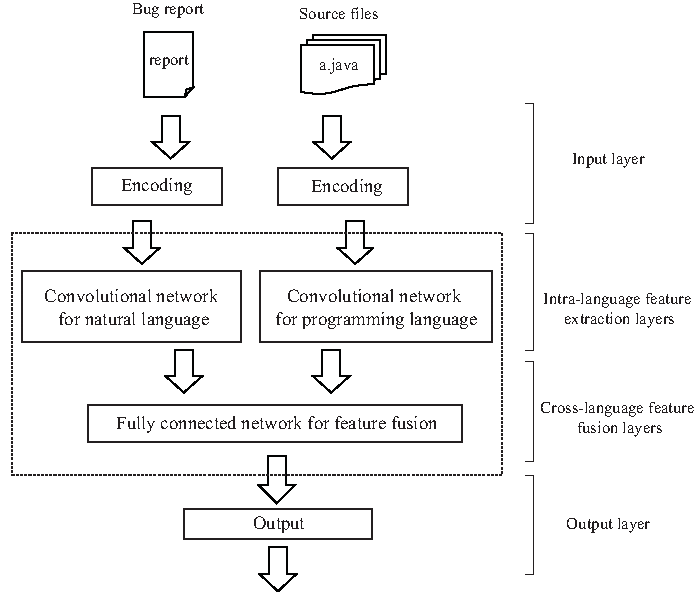
\includegraphics[width = \columnwidth]{pic/NPCNN-structure.pdf}
\caption{The general structure of Natural and Programming language Convolutional Neural Network.}
\label{fig:npcnn-structure}
\end{figure}

Huo et al. found that programming language %, although in textual format,
differs from natural language in two aspects. First, the basic language component carrying meaningful semantics in natural language is word or term, while the basic language component carrying meaningful semantics in programming language is statement. Second, natural language organizes words in a ``flat'' way while programming language organizes its statements in a ``structured'' way to produce richer semantics. Therefore, the structure of CNN for programming language, as shown in Figure~\ref{fig:npcnn}, is specifically designed to solve these two points. The first convolutional and pooling layers extract within-statements features while preserving the integrity of statements by sliding convolutional window within statements. The subsequent convolutional and pooling layers extract between-statements features reflecting the structural nature of code by employing convolutional window of different sizes. More details can be referred to in~\cite{huo2016learning}.

\begin{figure}[hbt]
\centering
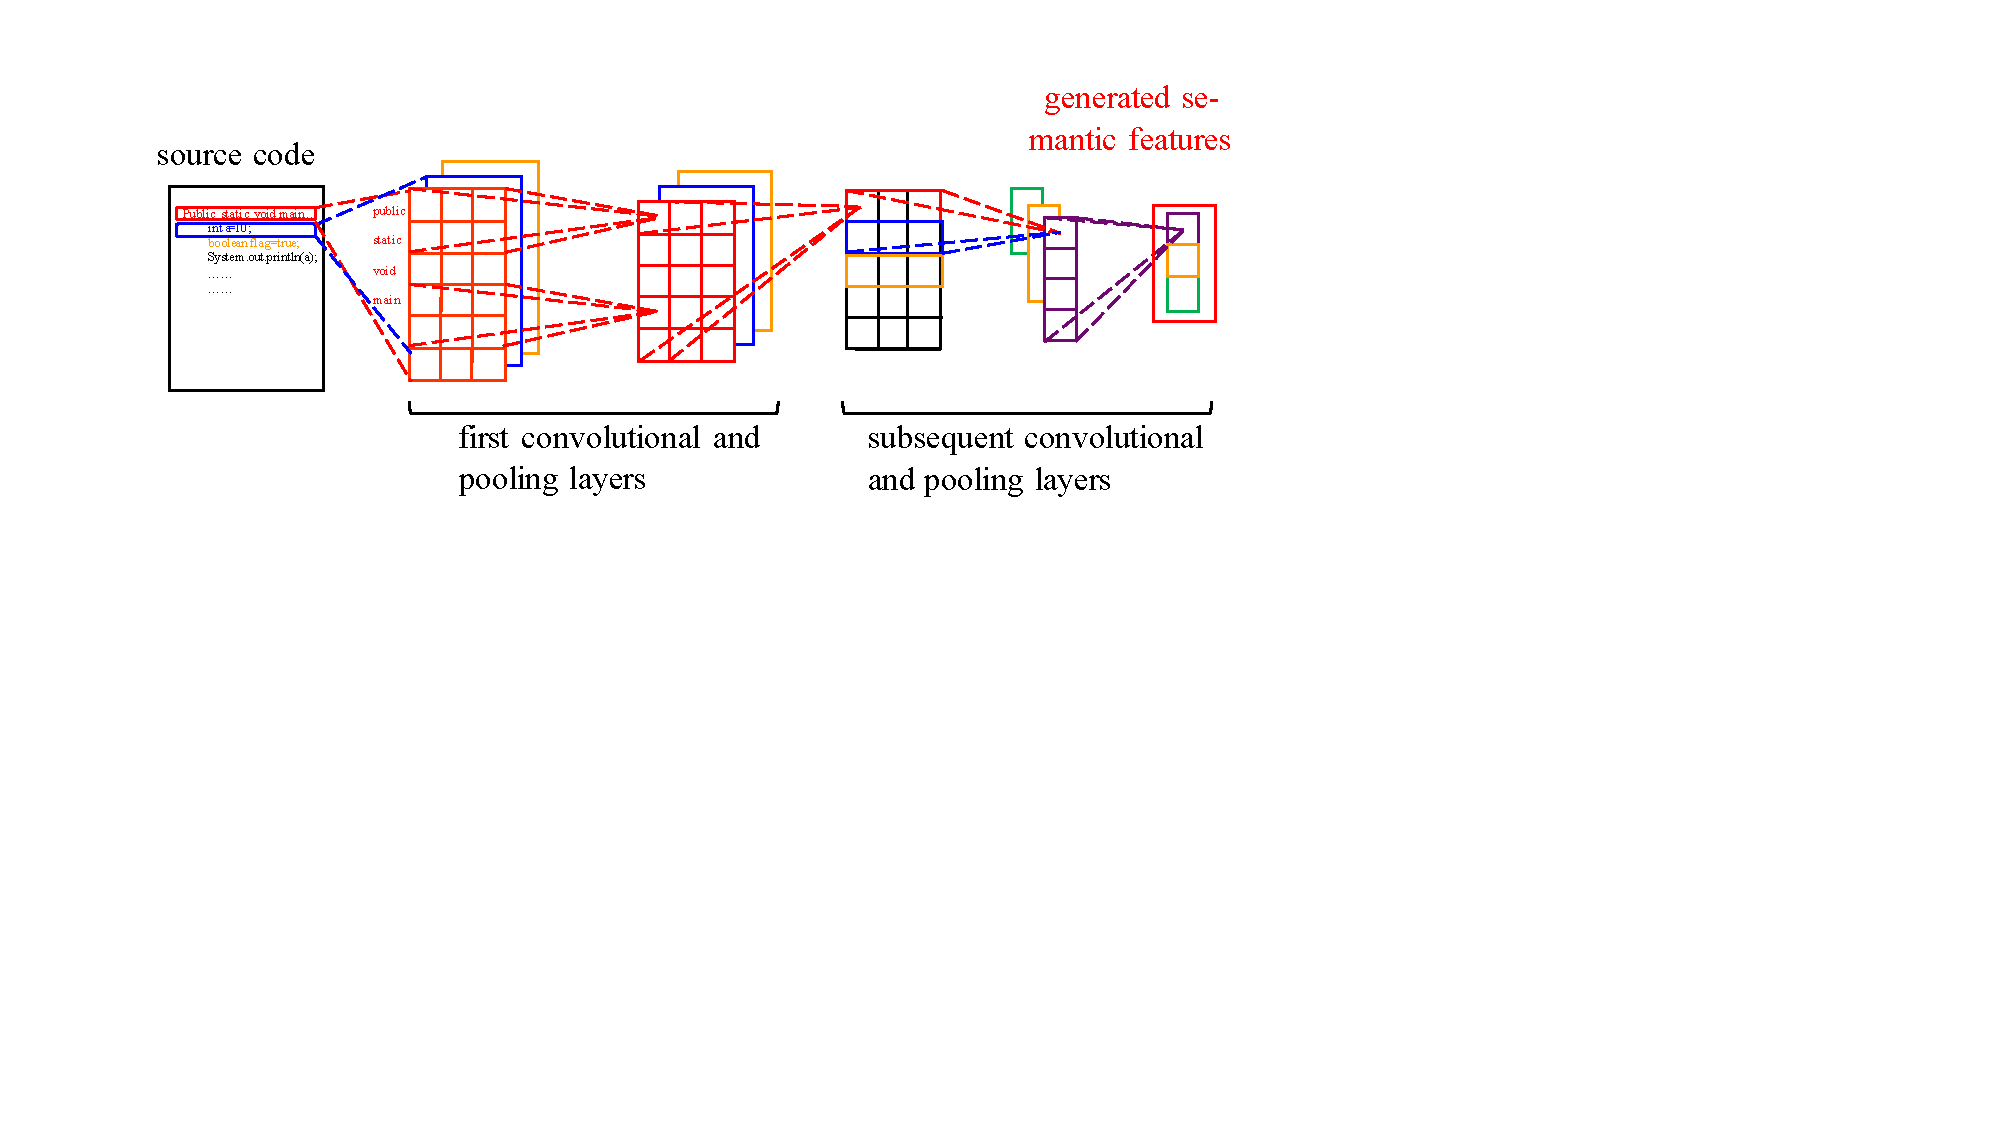
\includegraphics[width = \columnwidth]{pic/NPCNN.pdf}
\caption{The structure of convolutional neural network for programming language.}
\label{fig:npcnn}
\end{figure}

After feature extraction, the middle-level features generated from bug reports and source code are fed into the cross-language feature fusion layers. To deal with the imbalance nature of bug localization data, the cross-language feature fusion layers introduce an unequal misclassification cost according to a imbalance ratio between buggy and non-buggy files, and train a fully connected network in a cost sensitive manner. Let $cost_n$ denotes the cost of incorrectly associating an irrelevant source code file to a bug report and $cost_p$ denotes the cost of missing a buggy source code file that is responsible for the reported bugs. The weights of the fully connected networks $w$ can be learned by minimizing the following objective function using SGD (Stochastic Gradient Descent).
\begin{equation}
\begin{aligned}
\label{eq:cost2}
\mathop{\min}_{\mathbf{w}}\sum_{i,j}{[cost_n L(\mathbf{z}^{r}_i, \mathbf{z}^{c}_j, y_{ij}; \mathbf{w})(1-y_{ij})} \\
 {+cost_p L(\mathbf{z}^{r}_i, \mathbf{z}^{c}_i, y_{ij}; \mathbf{w})(1+y_{ij})]}+\lambda||\mathbf{w}||^2
\end{aligned}
\end{equation}



\section{Proposed Approach}\label{sec.approach}
\begin{figure*}[hbt]
\centering
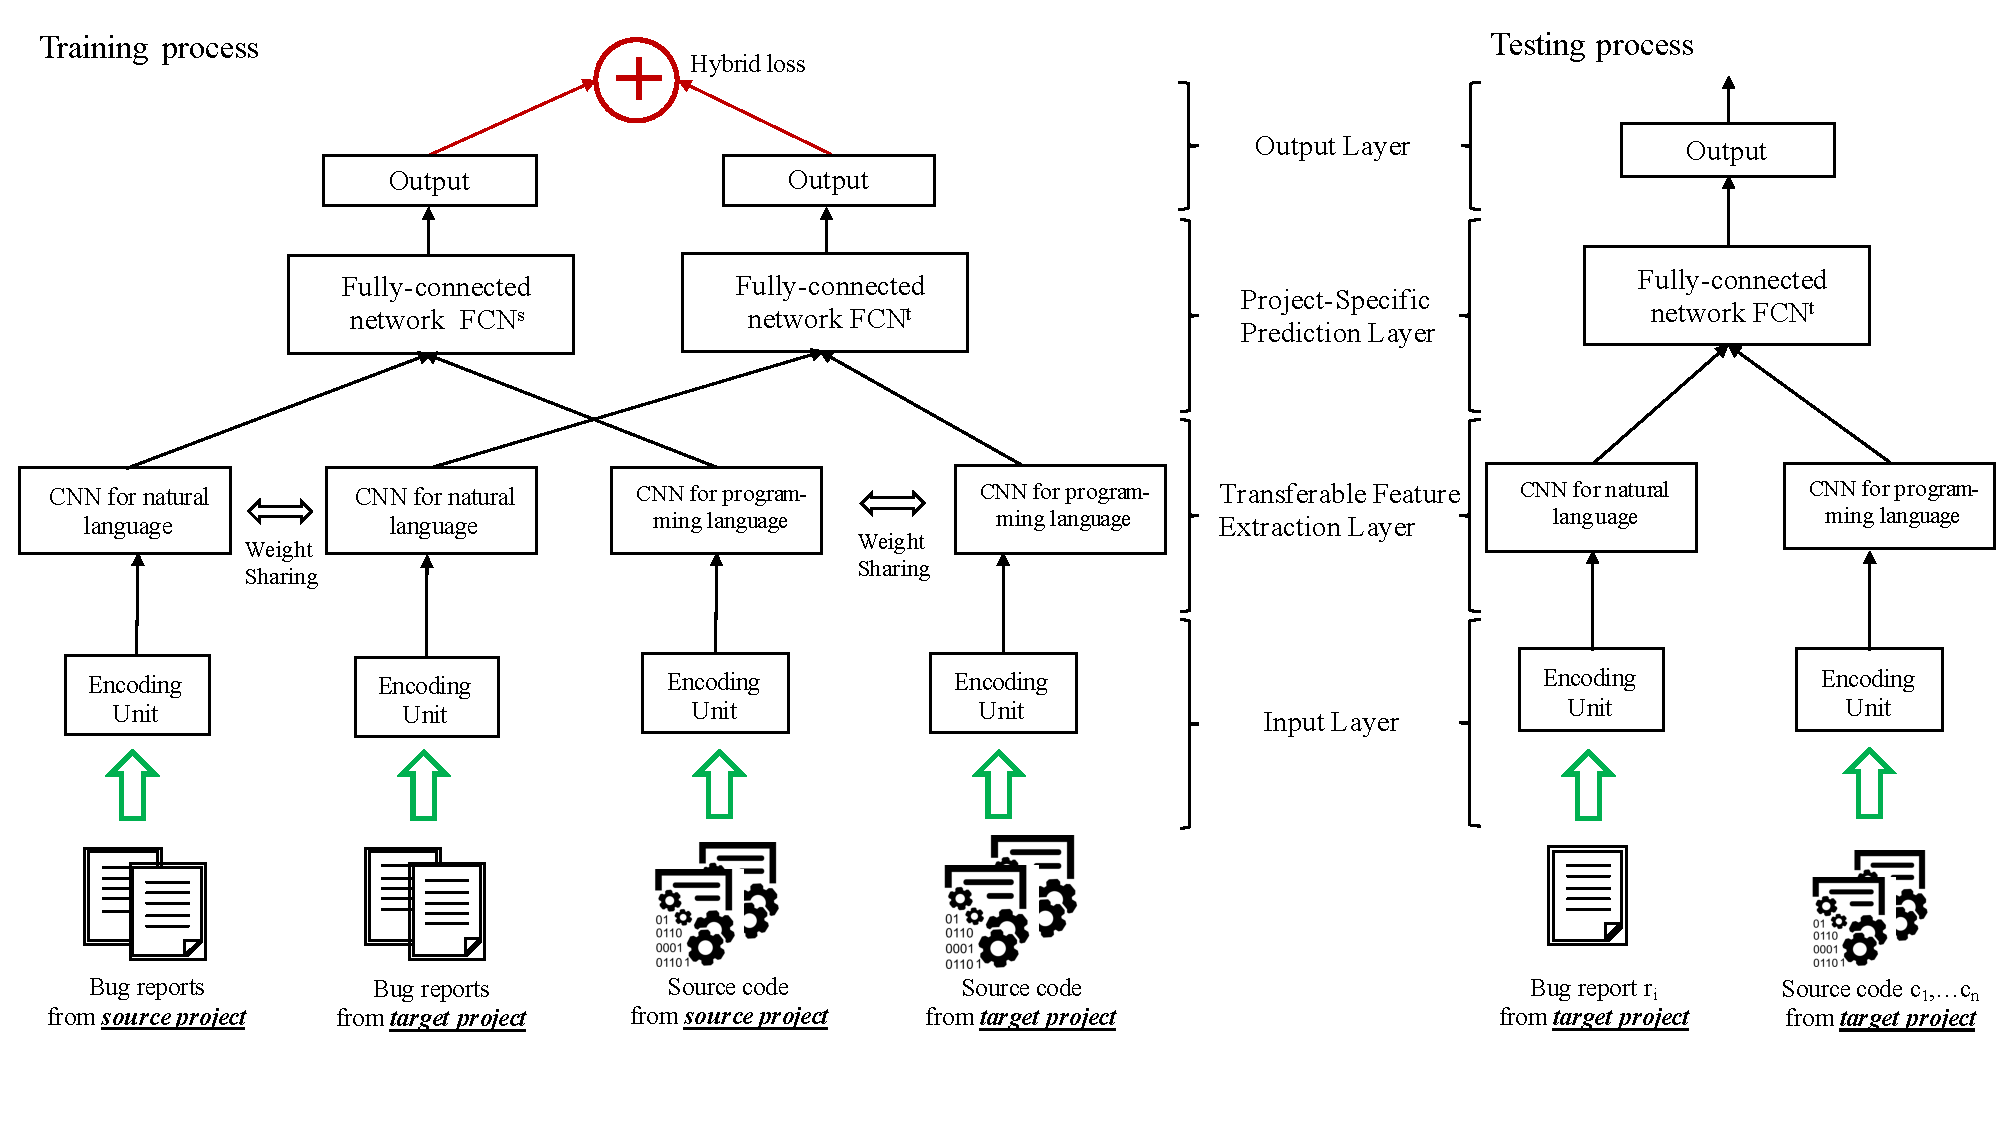
\includegraphics[width = 2\columnwidth]{pic/structure.pdf}
\caption{The overall structure of Transfer Natural and Programming language CNN.  The left part is the training process of \TRANPCNN based on the bug reports and source code from source projects and a few data from target projects, the weights of which are trained by minimizing the loss of ensemble loss from fully-connected networks $fc_s$ and $fc_t$. The right part is the testing process, a new bug report and its candidate source code are fed into the model, and \TRANPCNN outputs their relevant scores for bug localization.}
\label{fig:structure}
\end{figure*}

The goal of cross-project bug localization is using data from source project and a few data from target project to locate the potentially buggy source code in the target project that produce the program behaviors specified in a
given bug report. Let $\mathcal{C}_s =\{ c_{s_1}, c_{s_2}, \cdots, c_{s_{nc_1}}\}$ and $\mathcal{C}_t =\{ c_{t_1}, c_{t_2}, \cdots, c_{t_{nc_2}}\}$ denote the set of source code from source project and target project respectively, $\mathcal{C}=\mathcal{C}_s \bigcup \mathcal{C}_t $. $\mathcal{R}_s =\{ r_{s_1}, r_{s_2}, \cdots, r_{s_{nr_1}}\}$ and $\mathcal{R}_t =\{ r_{t_1}, r_{t_2}, \cdots, r_{t_{nr_1}}\}$ denotes the bug reports, respectively, $\mathcal{R}=\mathcal{R}_s \bigcup \mathcal{R}_t $, where $nc_1, nc_2, nr_1, nr_2$ denote the number of source files and bug reports from source project and target project, respectively. We formulate cross-project bug localization as a learning task which aims to learn a prediction function $f: \mathcal{R} \times \mathcal{C} \mapsto \mathcal{Y}$. $y_{ij} \in \mathcal{Y} = \{+1, -1 \}$ indicates whether a source code $c_j \in \mathcal{C} $ is relevant to a bug report $r_i \in \mathcal{R}$.

In this paper, we propose a novel deep transfer neural network named \TRANPCNN (TRAnsfer Natural and Programm Language Convolutional Neural Network) to instantiate the cross-project bug localization problem, which is an extension of NP-CNN proposed by Huo et al. \TRANPCNN takes the raw data of bug reports and source code as inputs and learns a unified feature mapping $\phi(\cdot, \cdot)$ for a given $r_i$ and $c_j$, based on which the prediction can be made with a subsequent output layer. We will introduce the general framework of \TRANPCNN and explain the way to employ deep transfer technique for cross-project bug localization in the following subsections.

\subsection{General Structure}
The general structure of \TRANPCNN is shown in Figure~\ref{fig:structure}. Specifically, \TRANPCNN consists of four parts: input layer, transferable feature extraction layers, heterogeneous predicting adaptation layers and output layer. The left figure indicates the training process of \TRANPCNN and the right figure indicates the test process. Since the \TRANPCNN model is used to deal with cross-project bug localization tasks, during the training process, pairs of source code and bug reports and ground truth labels from source project are fed into the deep neural network for weight training, as well as very few data from target project, and for testing process, a new bug report from target project and its candidate source code are fed into the model, which outputs their relevant scores indicating which code have high relevance to the given bug report and are located as buggy.



\subsection{Transferable Feature Extraction Layers}
Before processing in Transferable Feature Extraction Layers, the source code and bug reports should be firstly encoded as feature vectors. Traditional techniques usually employs TFIDF to represent text content, which may lose the word relationships. In our model, to maintain the semantics with structural information of text, we apply word2vec technique to encode bug reports and source code.

To process the bug reports in natural language, we follow the standard convolutional neural network~\cite{kim2014convolutional} (named as NCNN) to extract semantic features $\mathbf{h}^r$ from bug reports, which has been widely studied. Meanwhile, as mentioned in Huo et al.~\cite{huo2016learning}, bug reports and source code should be processed in different ways, because two languages have different structural semantic property. Therefore, we apply programming language specific convolutional neural network (named as PCNN) to extract semantic features from source code. The PCNN is able to preserve the integrity within statements by sliding convolutional windows within statements in the first convolutional and pooling layers, and generates semantic features between statements by applying  different sizes of convolutional windows in the subsequent convolutional and pooling layers. The details of PCNN is introduced in the background section and more details can be referred in Huo et al.'s work~\cite{huo2016learning}.

%Source code in programming language, although in textural format, differs from natural language mainly in two aspects. First, the basic language component carrying meaningful semantics in natural language is word or term, and the semantics of the natural language can be inferred from a bag of words. By contrast, in programming language the basic language component carrying meaningful semantics is statement, and the semantics of the programming language can be inferred from the semantics on multiple statements plus the way how these statements interact with each other along the execution path. Thus, to extract features from programming language, the convolution operations should explicitly respect to the atomicity of statements in semantics. Second, natural language organizes words in a ``flat'' way while programming language organizes its statements in a ``structured'' way to produce richer semantics. For example, a branching structure ``if-then-else'' defines two parallel groups of statements. Each group interacts with the statements before and after the branching block while there is no interaction between the two groups. Thus, to extract features from programming language, the convolution operations should obey the program structure defined by the programming languages.

Although the data distribution of cross-projects may be different, the semantics within the statements may be similar since the projects are using the same programming language so that the rule of semantic feature extraction is transferable. Therefore, in the training process, the PCNN models in the transferable feature extraction layers for processing source projects data and target projects data share the same parameter weights, which means that the rule to extract semantic features from programming languages are the same. This structure helps generate semantic features from target project using the large number of training source code in the source projects, leading to a better feature representation in the cross-project bug localization. 
 
\subsection{Heterogeneous Predicting Adaptation Layers}
After processing from transferable feature extraction layers, the high-level semantic features from bug reports and source code are extracted, which would be then fed into a fully-connected neural network for feature fusion. However, in cross-project bug localization, the data distribution of source project and target project is different, which means directly employing the same fully-connected network to fuse features from both source and target projects will have bias, leading to a poor bug localization performance.

One question arises here: can we design a particular network to extract features within project, and fuse feature in separate structure? To address this problem, we design two particular fully-connected networks to combine the middle-level features in Cross-project feature fusion layers: One fully-connected network $fc_s$ is used for source project feature fusion and the other fully-connected work $fc_t$ is used to fuse features in the target project. The structure suggests that the feature extraction of different projects are similar and can be processed in the same Convolutional Neural Network, and the feature fusion and projection process is different so that two separate fully-connected neural network are designed to solve this problem. The objective function in the cross-project feature fusion layers can be rewritten in Eq.~(\ref{eq:lossfunction}):
\begin{equation}
\begin{aligned}
\label{eq:lossfunction}
\mathop{\arg\min}_{\mathbf{W}}&\sum_{s_i,s_j}\mathcal{L}(\mathbf{h}_{s_i},\mathbf{h}_{s_j}
,y_{s_{ij}}; W_{fc_s}, W_{conv} ))\\
+&\sum_{t_i,t_j}\mathcal{L}(\mathbf{h}_{t_i},\mathbf{h}_{t_j},y_{t_{ij}}; W_{fc_t}, W_{conv})+\lambda||\mathbf{W}||^2
\end{aligned}
\end{equation}
where, $\mathcal{L}$ is the square loss, $\lambda$ is the trade-off parameter and the weight vectors $W$ contains the weight vectors in convolutional neural networks $W_{conv}$, in fully-connected network of source domain $W_{fc_s}$ and in fully-connected network of target domain $W_{fc_t}$. All the weights is learned by minimizing the objective function based on SGD (stochastic gradient descent) in the same time.


%cross-language feature fusion layers, where a fully-connected network is employed for learning a unified features and followed by an output layer mapping to the predictions $\mathcal{Y}$. However, a reported bug may only relevant to one or a few source code, while a large number of source code are irrelevant and this imbalance nature should be considered. Similar to~\cite{huo2016learning} which introduced an unequal misclassification cost to handle imbalance problem, we randomly drop some negative instances in the cross-language feature fusion layer, which can decrease the computational cost and counteract the negative influence of the imbalance nature. Let $y_{i}^{(k)}$ denote the $k$-th label of instance $\mathbf{x}_i$ and $\tilde{y}_{i}^{(k)}$ denote its prediction, similar to traditional LSTM model, we use cross entropy error function in the output layer, and the parameters are learned by minimizing the following loss function using stochastic gradient descent (SGD) method: 

\section{Experiments}\label{sec.exp}
To evaluate the effectiveness of \TRANPCNN, we conduct experiments on open source software projects and compare it with several state-of-the-art bug localization methods.

\subsection{Research Questions}
%\dl{Ferdian, please add details on why the RQs are interesting and the purpose of the RQs}

Our experiments are designed to address the following research questions:

\vspace{0.2cm}\noindent\textit{\textbf{RQ1}: Is there a need for a specialized technique for cross-project bug localization?}

If a model learned from one project can be used for other projects, then there is no need for a specialized technique for cross-project bug localization. Thus, before we consider other research questions, we validate the need for our proposed approach by empirically evaluating the effectiveness of a model learned from one project to localize bugs in other projects.

\vspace{0.2cm}\noindent\textit{\textbf{RQ2}: Do the project-specific prediction layer improve the bug localization performance?}

%\dl{Xuan, please help to motivate this research question. I can't motivate it since I believe the details of the approach is going to change.}

In Section 3, we propose to employ project-specific prediction layer that apply two fully-connected networks for prediction from source and target projects separately, which is the key part of \TRANPCNN. In this research question, we evaluate whether the layer improves the bug localization performance by comparing the results with NP-CNN.

\vspace{0.2cm}\noindent\textit{\textbf{RQ3}: Can \TRANPCNN outperform other bug localization methods?}

A number of bug localization methods have been proposed in the literature. In this research question, we evaluate whether and to what extent can our proposed approach \TRANPCNN outperforms the state-of-the-art methods designed for bug localization and those that can be adapted for bug localization. 

\subsection{Datasets}
We consider three datasets containing a total of 5,591 reports from JIRA issue tracking systems of HTTPClient (H)\footnote{\url{http://hc.apache.org/httpcomponents-client-ga/index.html}}, Jackrabbit (J)\footnote{\url{https://jackrabbit.apache.org/jcr/index.html}}, and Lucene-Java (L)\footnote{\url{ http://lucene.apache.org/}}. HTTPClient is a library for implementing the client side of HTTP standard, while Jackrabbit is a content repository, and Lucene is a text search engine. We only consider projects with JIRA issue tracking systems since links between bug reports and their bug fixing commits stored in them are typically more reliable than those stored in Bugzilla issue tracking systems -- c.f.,~\cite{BissyandeTWLJR13}. The details of the reports considered in this study are shown in Table~\ref{tab:reports} and they have been used before by Kochhar et al.~\cite{KochharTL14}. 

\begin{table}
\caption{Bug Report Dataset}\label{tab:reports}
\begin{tabular}{|l|l|l}
\hline
{\bf Project} & {\bf \# Reports} \\
\hline HTTPClient & 746\\
\hline Jackrabbit & 2,402\\
\hline Lucene-Java & 2,443\\
\hline
\end{tabular}
\end{table}

\dl{Xuan, I thought we are also using your previous datasets? If we only use Pavneet's dataset, do we use all of them or only some of them that are not biased? Pavneet showed that some of the dataset is biased ... reviewers may be concerned with this bias ... Bias 2 mentioned in this paper (\url{http://ink.library.smu.edu.sg/cgi/viewcontent.cgi?article=3425&context=sis_research}) is particularly important.}

\xh{Currently we only use Paveneet's datasets (H,J and L), and yes we have considered the bias, and we only use the unbiased data sets. The ``fully localized'' bug reports are filtered. Our previous data sets are bias, so we are not sure if we use here is suitable.  If necessary, we can conduct several comparison experiments ono more data sets. }

%\dl{Ferdian, please add details datasets. Please see the following papers for details of the datasets:~\cite{huo2016learning,KochharTL14}.}



\subsection{Evaluation Metrics}
%The evaluation metrics are presented here. %\dl{Ferdian, please add details on evaluation metrics.}

Following prior bug localization studies~\cite{SahaLKP13,SahaLKP14,zhou2012should,huo2016learning}, we consider three evaluation metrics: Top-N, Mean Average Precision (MAP), and Mean Reciprocal Rank. Their brief definitions considering the context of bug localization are given below:

\vspace{0.2cm}\noindent{\bf Top-N.} Top-N reports the proportion of bug reports for which one of the buggy files appear in the top-N position in the ranked list returned by a bug localization tool. Following prior studies~\cite{SahaLKP13,SahaLKP14,zhou2012should,huo2016learning}, we consider three values of N, i.e., 1, 5, and 10. This is further motivated by the findings of Kochhar et al.~\cite{KochharXLL16} which highlight that more than 95\% of practitioners would not check beyond the top-10 results of a bug localization tool.

\vspace{0.2cm}\noindent{\bf Mean Average Precision (MAP).} For each ranked list produced by a bug localization technique for a bug report, we can compute its average precision (AP) as follows:

\begin{equation}
\sum_{i} \frac{P(i)\times isBuggy(i)}{\# buggy files}
\end{equation}

In the above equation, $\mathit{P(i)}$ is the precision at position $i$ (i.e., proportion of files at position 1 to $i$ that are buggy), while $\mathit{isBuggy(i)}$ is 1 if the file at position $i$ is buggy and 0 otherwise. The denominator of the equation is the number of buggy files in the entire ranked list. MAP is the mean of APs considering all bug reports.

\vspace{0.2cm}\noindent{\bf Mean Reciprocal Rank (MRR).} For each ranked list produced by a bug localization technique for a bug report, we can compute the position of the first buggy file. The reciprocal of such position is referred to as the reciprocal rank (RR). MRR is the mean of RRs considering all bug reports.



\subsection{Baselines}

We compare our proposed model \TRANPCNN with following baseline methods:
\begin{itemize}
  \item VSM (Vector Space Model)~\cite{rao2011retrieval}: a baseline method that firstly uses Vector Space Model to represent the text bug reports and source code, then employs Logistic Regression to predict the related buggy source code.
  \item Burak (Burak Filter)~\cite{peters2013better}: a state-of-the-art method for cross-project and cross-company defect prediction problem, which filters training sets using Burak filter that employs k-nearest neighbour to selects instances in the source project similar to the test project.
  \item TCA-R (Transfer Component Analysis with Logistic Regression): a state-of-the-art transfer learning method in software engineering, which firstly employ TCA to map source and target project into a same feature space and then apply Logistic Regression for bug localization (same settings suggested in their paper). 
  \item TCA-P (Transfer Component Analysis with Multi-layer Perceptron): a state-of-the-art transfer learning method in software engineering, which firstly employ TCA to map source and target project into a same feature space and then apply MLPs for bug localization (same settings with fully-connected layers in \TRANPCNN).
   \item TCA-D (Transfer Component Analysis with Deep features): a state-of-the-art transfer learning method in software engineering, which firstly employ TCA to map source and target project into a same feature space and then apply Logistic Regression for bug localization (using deep features extracted from CNN instead of TFIDF features).
  \item NP-CNN (Natural and Programming language Convolutional Neural Network)~\cite{huo2016learning}: a state-of-the-art deep model for bug localization, which use source project data for training and localizing the buggy source code for target project data.
%  \item SimpleTrans (Simple Transfer): a variant of the \TRANPCNN model, which trains the prediction model on the source project data, and use fine tune method for weight adjustment based on the target project.
\end{itemize}
\ft{Settings would probably better be grouped in experimental settings section. There is no citation for TCA. }

\subsection{Experimental Settings}

For parameter settings of baseline methods, we use the same parameter settings suggested in their work~\cite{rao2011retrieval}. For the \TRANPCNN model, we employ the most commonly used ReLU $\sigma(x)=\max(0,x)$ as active function and the filter windows size $d$ is set as 3, 4, 5, with 100 feature maps each in Within-Project feature extraction layers. The number of neurons in fully-connect network in  set the same number of CNN. In addition, the drop-out method is also applied which is used to prevent co-adaption of hidden units by randomly dropping out values in fully-connected layers, and the drop-out probability $p$ is set 0.25 in our experiments.

For data partition, we use data from source projects and 20\% target projects as training sets, and locates the 80\% buggy code in target projects. This process repeats for 5 times to reduce the influence of randomness, and we report the average results in the next section.

\section{Experimental Results}

\subsection{Experimental Results for Research Questions}

\begin{table}[htbp]
  \centering
  \caption{Performance Comparisons between within-project and cross-project bug localization.}
  \resizebox{!}{0.5\columnwidth}{
    \begin{tabular}{c|l|c|c|c|c|c}
    \toprule
    Tasks & \textit{Methods} & \multicolumn{1}{l}{\textit{Top 1}} & \multicolumn{1}{l}{\textit{Top 5}} & \multicolumn{1}{l}{\textit{Top 10}} & \multicolumn{1}{l}{\textit{MAP}} & \multicolumn{1}{l}{\textit{MRR}} \\
    \midrule
    \multirow{3}[0]{*}{\textbf{J}$\rightarrow$\textbf{H}} & NPCNN & 0.317  & 0.362  & 0.508  & 0.276  & 0.352  \\
          & NPCNN$^{partial}$ & 0.204  & 0.258  & 0.313  & 0.202  & 0.292  \\
          & NPCNN$^{full}$ & 0.533  & 0.617  & 0.650  & 0.472  & 0.580  \\
          \midrule
    \multirow{3}[0]{*}{\textbf{L}$\rightarrow$\textbf{H}} & NPCNN & 0.142  & 0.192  & 0.345  & 0.161  & 0.218  \\
          & NPCNN$^{partial}$ & 0.204  & 0.258  & 0.313  & 0.202  & 0.292  \\
          & NPCNN$^{full}$ & 0.533  & 0.617  & 0.650  & 0.472  & 0.580  \\
          \midrule
    \multirow{3}[0]{*}{\textbf{H}$\rightarrow$\textbf{J}} & NPCNN & 0.167  & 0.287  & 0.349  & 0.247  & 0.277  \\
          & NPCNN$^{partial}$ & 0.035  & 0.211  & 0.302  & 0.155  & 0.189  \\
          & NPCNN$^{full}$ & 0.508  & 0.587  & 0.679  & 0.462  & 0.557  \\
          \midrule
    \multirow{3}[0]{*}{\textbf{L}$\rightarrow$\textbf{J}} & NPCNN & 0.152  & 0.182  & 0.318  & 0.176  & 0.221  \\
          & NPCNN$^{partial}$ & 0.035  & 0.211  & 0.302  & 0.155  & 0.189  \\
          & NPCNN$^{full}$ & 0.508  & 0.587  & 0.679  & 0.462  & 0.557  \\
          \midrule
    \multirow{3}[0]{*}{\textbf{H}$\rightarrow$\textbf{L}} & NPCNN & 0.173  & 0.246  & 0.390  & 0.196  & 0.329  \\
          & NPCNN$^{partial}$ & 0.097  & 0.219  & 0.335  & 0.095  & 0.109  \\
          & NPCNN$^{full}$ & 0.289  & 0.484  & 0.611  & 0.287  & 0.387  \\
          \midrule
    \multirow{3}[0]{*}{\textbf{J}$\rightarrow$\textbf{L}} & NPCNN & 0.110  & 0.255  & 0.323  & 0.141  & 0.176  \\
          & NPCNN$^{partial}$ & 0.097  & 0.219  & 0.335  & 0.095  & 0.109  \\
          & NPCNN$^{full}$ & 0.289  & 0.484  & 0.611  & 0.287  & 0.387  \\
%          \midrule
%    \multirow{3}[0]{*}{Avg.} & NPCNN & 0.177  & 0.254  & 0.372  & 0.200  & 0.262  \\
%          & NPCNN$^{partial}$ & 0.112  & 0.229  & 0.317  & 0.151  & 0.197  \\
%          & NPCNN$^{full}$ & 0.443  & 0.563  & 0.647  & 0.407  & 0.508  \\
          \bottomrule
    \end{tabular}%
    }

  \label{tab:within}%
\end{table}%


\begin{figure}[hbt]
\centering
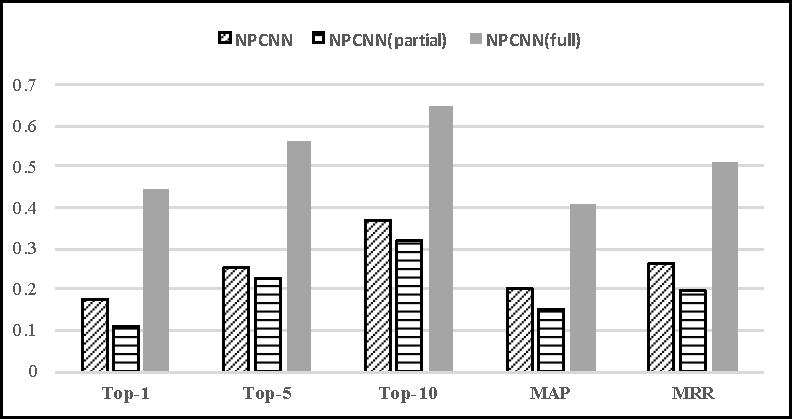
\includegraphics[width = 0.9\columnwidth]{pic/results1.pdf}
\caption{Performance comparisons between within-project and ross-project bug localization.}
\label{fig:results1}
\end{figure}


\textbf{RQ1}: \textit{Is there a need for cross-project bug localization?}

To answer this research question, we compare the results of using NP-CNN for bug localization in different settings.

\begin{itemize}
  \item NPCNN: Employ NPCNN directly for cross-project bug localization, which means directly training the model on the data from source projects and locating the bugs in the target project.
  \item NPCNN$^{partial}$: Employ NPCNN using partial data of target projects, which means training based on a few data (20\%) in the target projects, and localizes target buggy files without using data from source project.
  \item NPCNN$^{full}$: Employ NPCNN using full data of target projects. In this setting, we conduct 5-folds cross-validation for comparison.
\end{itemize}

The results are detailed in Tab.~\ref{tab:within}\ft{Tab. should be Table. The same throughout the paper.}. There are six tasks in the table, in which $\textbf{H}$ represents project \textit{httpclient}, $\textbf{J}$ represents project \textit{jackrabbit} and $\textbf{L}$ represents \textit{lucene-solr}. Meanwhile, the task $\textbf{H} \rightarrow \textbf{J}$ represents using \textit{httpclient} as source project and predicts the location of buggy files in target project \textit{jackrabbit}.\ft{Project name should be capitalized properly following Table~\ref{tab:reports}. lucene-solr should be Lucene-Java.} The results show that the performance of bug localization using full data of target projects is the best, which has a large gap against the performance using partial data. For cross-project bug localization, the performance of NPCNN that directly uses source projects is better than NPCNN$^{within}$\ft{What is NPCNN$^{within}$?}, showing that cross-project data is beneficial to improve the bug localization performance, but directly using within-project bug localization technique will not as well as NPCNN$^{full}$. The results suggest that there is a need for cross-project bug localization, and directly using within-project bug localization method does not show good performance.

\textbf{RQ2}: \textit{Do the heterogeneous predicting adaptation layers improve the bug localization performance?}

To answer this research question, we compare the results of \TRANPCNN with the original NPCNN. The difference of the structure between \TRANPCNN and NPCNN is that \TRANPCNN employs two fully-connected networks to combine deep features from source projects and target projects in the heterogeneous predicting adaptation layers, respectively, which will counter the influences that cross-project data may have different distribution leading to a bias performance. The results are detailed in Tab.~\ref{tab:results2}.

\ft{It would be good if we can explain why such structure can counter bias. Perhaps we should explain this first in approach (theory) and then highlight it again accompanied with experimental result (empirical).}

%According to the results, we find that SimpleTrans improves a little performance against NPCNN, showing that transfer technique is effective in improving cross-project bug localization performance. Meanwhile, it can be obviously found that \TRANPCNN performs better than NPCNN in terms of all evaluation metrics, which shows that the structure of cross-project feature fusion layer is able to improve cross-project bug localization performance.

\begin{table}[htbp]
  \centering
  \caption{Performance Comparisons with previous deep models.}
  \resizebox{!}{0.35\columnwidth}{
    \begin{tabular}{c|l|c|c|c|c|c}
    \toprule
    Tasks & \textit{Methods} & \textit{Top 1} & \textit{Top 5} & \textit{Top 10} & \textit{MAP} & \textit{MRR} \\
    \midrule
    \multirow{2}[0]{*}{\textbf{J}$\rightarrow$\textbf{H}} & NPCNN & 0.317  & 0.362  & 0.508  & 0.276  & 0.352  \\
%          & SimpleTrans & 0.354 & 0.396 & 0.563 & 0.298 & 0.395 \\
          & \TRANPCNN & 0.500   & 0.583 & 0.625 & 0.376 & 0.543 \\
          \midrule
    \multirow{2}[0]{*}{\textbf{L}$\rightarrow$\textbf{H}} & NPCNN & 0.142  & 0.192  & 0.345  & 0.161  & 0.218  \\
%          & SimpleTrans & 0.163 & 0.146 & 0.354 & 0.141 & 0.246 \\
          & \TRANPCNN & 0.275 & 0.35  & 0.488 & 0.242 & 0.332 \\
          \midrule
    \multirow{2}[0]{*}{\textbf{H}$\rightarrow$\textbf{J}} & NPCNN & 0.167  & 0.287  & 0.349  & 0.247  & 0.277  \\
%          & SimpleTrans & 0.133 & 0.324 & 0.365 & 0.273 & 0.301 \\
          & \TRANPCNN & 0.396 & 0.443 & 0.514 & 0.371 & 0.434 \\
          \midrule
    \multirow{2}[0]{*}{\textbf{L}$\rightarrow$\textbf{J}} & NPCNN & 0.152  & 0.182  & 0.318  & 0.176  & 0.221  \\
%          & SimpleTrans & 0.144 & 0.204 & 0.382 & 0.247 & 0.249 \\
          & \TRANPCNN & 0.460  & 0.462 & 0.488 & 0.404 & 0.478 \\
          \midrule
    \multirow{2}[0]{*}{\textbf{H}$\rightarrow$\textbf{L}} & NPCNN & 0.173  & 0.246  & 0.390  & 0.196  & 0.329  \\
%          & SimpleTrans & 0.197 & 0.323 & 0.426 & 0.152 & 0.313 \\
          & \TRANPCNN & 0.361 & 0.445 & 0.535 & 0.279 & 0.414 \\
          \midrule
    \multirow{2}[0]{*}{\textbf{J}$\rightarrow$\textbf{L}} & NPCNN & 0.110  & 0.255  & 0.323  & 0.141  & 0.176  \\
%          & SimpleTrans & 0.140  & 0.282 & 0.342 & 0.163 & 0.224 \\
          & \TRANPCNN & 0.301 & 0.410  & 0.517 & 0.247 & 0.368 \\
%          \midrule
%    \multirow{3}[0]{*}{Avg.} & NPCNN & 0.177  & 0.254  & 0.372  & 0.200  & 0.262  \\
%          & SimpleTrans & 0.189  & 0.279  & 0.405  & 0.212  & 0.288  \\
%          & \TRANPCNN & 0.382  & 0.449  & 0.528  & 0.320  & 0.428  \\
          \bottomrule
    \end{tabular}%
    }
  \label{tab:results2}%
\end{table}%

\begin{figure}[hbt]
\centering
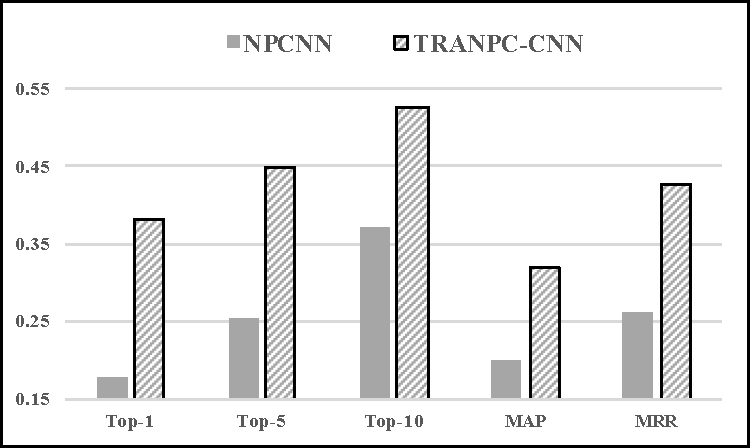
\includegraphics[width = 0.9\columnwidth]{pic/results2.pdf}
\caption{Performance comparisons with previous deep models.}
\label{fig:results2}
\end{figure}

The results show that \TRANPCNN performs better than NP-CNN, which suggests that the cross-projects feature fusion layers can improve the performance of cross-projects bug localization.

\textbf{RQ3}: \textit{Can \TRANPCNN outperform other bug localization methods?}

To answer this research question, we compare the results of \TRANPCNN with state-of-the-art methods: VSM (Vector Space Model), Burak (Burak Filter), TCA-R (Transfer Component Analysis with Logistic Regression), TCA-P (Transfer Component Analysis with Multi-layer Perceptron). Vector Space Model is a baseline technique used in the within-project bug localization and we employ it on cross-project bug localization for comparison. Burak and TCA have been shown good performance on cross-project and cross-company defect prediction, and also we apply it on cross-project bug localization. The parameters are set suggested in their work, i.e., $k=2$ in Burak method, and for TCA, we implement the algorithm with TCA+. For fair comparison, the classifier in their original paper (Logistic Regression) and multi-layer perception (same as \TRANPCNN) is compared in our experiments. The results are detailed in Tab.~\ref{tab:results3}. \ft{We should directly use abbreviations of baseline names since they have been introduced in Baselines section. Introduction of baselines are also redundant. }

According to the results, we have several findings: 1. Burak and TCA techniques perform better than the baseline VSM model, indicating that using transfer algorithms is able to improve the performance in cross-project bug localization; 2. \TRANPCNN outperforms TCA-P, which shows that the high-level features extracted from CNN are more semantic and informative, leading to a better representation and bug localization performance; 3. TCA-D uses deep features extracted from CNN and the performance is not as well as \TRANPCNN, which further proves that the cross-project feature fusion layers improve bug localization performance; 4. \TRANPCNN obtains the best average values in terms of all evaluation metrics, suggesting that \TRANPCNN outperforms other traditional bug localization methods and transfer techniques on software engineering.

\ft{We can highlight the amount of improvement that \TRANPCNN achieves as compared to the best baseline.}


% Table generated by Excel2LaTeX from sheet 'Sheet3'
\begin{table}[htbp]
  \centering
  \caption{Performance comparisons with traditional bug localization models.}
  \resizebox{!}{0.9\columnwidth}{
    \begin{tabular}{c|l|c|c|c|c|c}
    \toprule
    Tasks & \textit{Methods} & \multicolumn{1}{c|}{\textit{Top 1}} & \multicolumn{1}{c|}{\textit{Top 5}} & \multicolumn{1}{c|}{\textit{Top 10}} & \multicolumn{1}{c|}{\textit{MAP}} & \multicolumn{1}{c}{\textit{MRR}} \\
    \midrule
    \multirow{6}[0]{*}{\textbf{J}$\rightarrow$\textbf{H}} & VSM   & 0.098  & 0.157  & 0.177  & 0.087  & 0.143  \\
          & Burak & 0.110  & 0.126  & 0.138  & 0.116  & 0.121  \\
          & TCA-R & 0.120  & 0.212  & 0.144  & 0.157  & 0.162  \\
          & TCA-P & 0.114  & 0.133  & 0.154  & 0.123  & 0.176  \\
          & TCA-D & 0.122  & 0.225  & 0.271  & 0.168  & 0.248  \\
          & \TRANPCNN & 0.500  & 0.583  & 0.625  & 0.376  & 0.543  \\
          \midrule
    \multirow{6}[0]{*}{\textbf{L}$\rightarrow$\textbf{H}} & VSM   & 0.059  & 0.098  & 0.237  & 0.099  & 0.112  \\
          & Burak & 0.113  & 0.203  & 0.242  & 0.143  & 0.143  \\
          & TCA-R & 0.120  & 0.188  & 0.244  & 0.151  & 0.158  \\
          & TCA-P & 0.128  & 0.200  & 0.252  & 0.161  & 0.167  \\
          & TCA-D & 0.102  & 0.237  & 0.367  & 0.161  & 0.202  \\
          & \TRANPCNN & 0.275  & 0.350  & 0.488  & 0.242  & 0.332  \\
          \midrule
    \multirow{6}[0]{*}{\textbf{H}$\rightarrow$\textbf{J}} & VSM   & 0.035  & 0.211  & 0.232  & 0.165  & 0.129  \\
          & Burak & 0.130  & 0.150  & 0.206  & 0.225  & 0.195  \\
          & TCA-R & 0.115  & 0.162  & 0.209  & 0.239  & 0.244  \\
          & TCA-P & 0.114  & 0.154  & 0.203  & 0.237  & 0.241  \\
          & TCA-D & 0.111  & 0.135  & 0.157  & 0.168  & 0.185  \\
          & \TRANPCNN & 0.396  & 0.443  & 0.514  & 0.371  & 0.434  \\
          \midrule
    \multirow{6}[0]{*}{\textbf{L}$\rightarrow$\textbf{J}} & VSM   & 0.197  & 0.212  & 0.293  & 0.167  & 0.216  \\
          & Burak & 0.161  & 0.132  & 0.368  & 0.170  & 0.187  \\
          & TCA-R & 0.136  & 0.183  & 0.370  & 0.170  & 0.179  \\
          & TCA-P & 0.114  & 0.116  & 0.397  & 0.138  & 0.191  \\
          & TCA-D & 0.178  & 0.236  & 0.469  & 0.227  & 0.256  \\
          & \TRANPCNN & 0.460  & 0.462  & 0.488  & 0.404  & 0.478  \\
          \midrule
    \multirow{6}[0]{*}{\textbf{H}$\rightarrow$\textbf{L}} & VSM   & 0.083  & 0.278  & 0.393  & 0.154  & 0.136  \\
          & Burak & 0.105  & 0.226  & 0.272  & 0.123  & 0.222  \\
          & TCA-R & 0.136  & 0.208  & 0.383  & 0.170  & 0.279  \\
          & TCA-P & 0.143  & 0.226  & 0.394  & 0.171  & 0.288  \\
          & TCA-D & 0.162  & 0.207  & 0.345  & 0.229  & 0.292  \\
          & \TRANPCNN & 0.361  & 0.445  & 0.535  & 0.279  & 0.414  \\
          \midrule
    \multirow{6}[0]{*}{\textbf{J}$\rightarrow$\textbf{L}} & VSM   & 0.038  & 0.077  & 0.154  & 0.124  & 0.204  \\
          & Burak & 0.138  & 0.161  & 0.176  & 0.168  & 0.226  \\
          & TCA-R & 0.135  & 0.111  & 0.172  & 0.169  & 0.222  \\
          & TCA-P & 0.136  & 0.132  & 0.192  & 0.173  & 0.237  \\
          & TCA-D & 0.142  & 0.297  & 0.308  & 0.238  & 0.293  \\
          & \TRANPCNN & 0.301  & 0.410  & 0.517  & 0.247  & 0.368  \\
%          \midrule
%    \multirow{6}[0]{*}{Avg.} & VSM   & 0.085  & 0.172  & 0.248  & 0.133  & 0.157  \\
%          & Burak & 0.126  & 0.166  & 0.234  & 0.157  & 0.182  \\
%          & TCA-R & 0.127  & 0.178  & 0.254  & 0.176  & 0.207  \\
%          & TCA-P & 0.125  & 0.160  & 0.265  & 0.167  & 0.217  \\
%          & TCA-D & 0.136  & 0.223  & 0.319  & 0.199  & 0.246  \\
%          & \TRANPCNN & 0.382  & 0.449  & 0.528  & 0.320  & 0.428  \\
          \bottomrule
    \end{tabular}%
    }
  \label{tab:results3}%
\end{table}%

\begin{figure}[hbt]
\centering
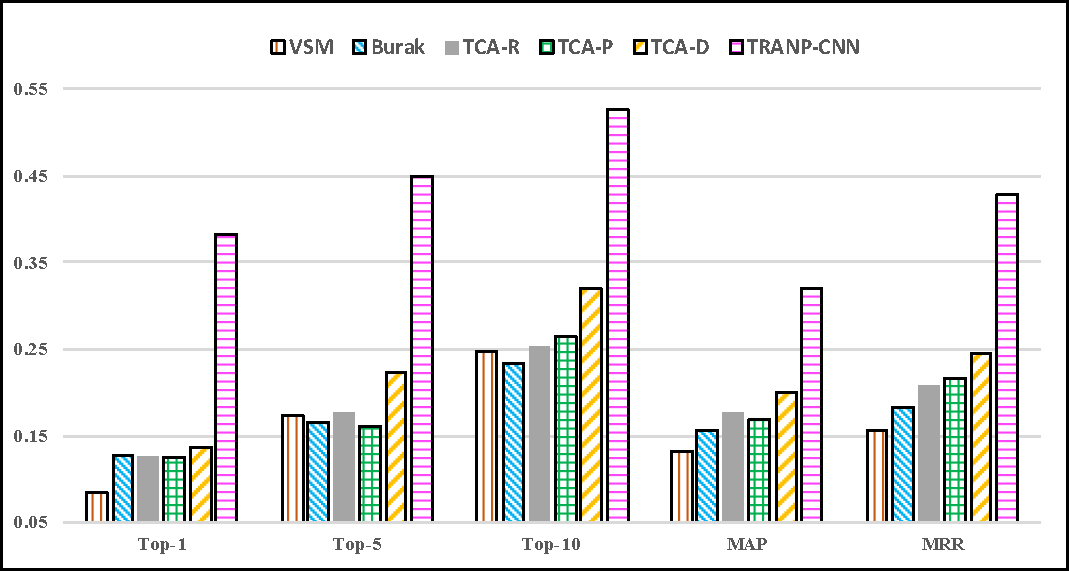
\includegraphics[width = 0.9\columnwidth]{pic/results3.pdf}
\caption{Performance comparisons with traditional bug localization models.}
\label{fig:results3}
\end{figure}



\section{Discussion}\label{sec.discuss}
\subsection{Why do the project-specific correlation fitting layers work? }
Firstly, we explore the reason why the project-specific correlation fitting layers in the \TRANPCNN model. The key part of \TRANPCNN is the project-specific correlation fitting layers, and in this section, we discuss why the project-specific correlation fitting layers work. 

The only difference between NP-CNN and \TRANPCNN is that the \TRANPCNN applies project-specific correlation fitting layers, which is particularly designed for cross-project bug localization to deal with the situation that the distribution of data from source project and target project are inconsistent, leading to a bias results if the prediction structure is the same. The \TRANPCNN model employs two fully-connected network for bug localization prediction, one is for source project and the other one is used for target project. This structure overcomes the problem that the model training from two projects affected from each other. During training process, the data of source project uses the CNN model in the transferable feature extraction layers  for feature extraction and employs the fully-connected network $fc^s$ for prediction training, and the target project data is trained using the same CNN but predicted with fully-connected network $fc^t$. This process helps improve the bug localization performance from target project by enjoying the advantage in sharing the same network of transferable feature extraction process from source project, and meanwhile adapting prediction network using training data from target project. 

\subsection{Why does \TRANPCNN improve the bug localization performance?}
The reason why \TRANPCNN improve the bug localization performance can be summarized as 4 folds:
\begin{itemize}
\item The transferable feature extraction layers are able to generate a more semantic representation of source code. The transferable feature extraction layers are able to extract the semantic features reflecting the structural and sequential nature, leading to a high-level representation of source code. In addition, the results in Table~\ref{tab:results3} that TCA+$^{(D)}$ (TCA+ with deep features) outperforms TCA+$^{(P)}$ (TCA+ with traditional features), which show that the deep features generated by transferable feature extraction layers are able to improve the performance of cross-project bug localization performance. 
\item The transferable feature extraction layers can improve the performance in cross-project bug localization. As aforementioned, since source project and target project use the same programming language, the semantic feature extraction rule of cross-project is similar, which means that the semantic feature extraction sub-structure from source project could be transferable to the target model. The comparison results between \TRANPCNN and NPCNN have supported this reason. 
\item The project-specific correlation fitting layers are effective for cross-project bug localization. The reason has been explained in the last subsection that the project-specific correlation fitting layers help counter the inconsistent distribution problems in cross-project bug localization task by employing two fully-connected network for predicting adaptation.
\item \TRANPCNN can fully exploit the advantage in using the labeled data from target project. A few data (20\% in our experiments) from the target project has labels. \TRANPCNN is able to make better use of labeled data from target project in training the fully-connected network $fc^t$ for prediction during the training process. However, traditional transfer model TCA+ has not fully used the labeled data in the target project from transfer learning view. 
\end{itemize}



\subsection{Threats to Validity}

There are three kinds of threat that may impact the validity of this study: threats to internal validity, threats to external validity, and threats to construct validity. We acknowledge these threats below.

Threats to internal validity relate to author bias and errors in our code and experiments. We have checked our code for bugs and fixed any that we can identify. There may still be errors that we do not notice though. The dataset that we obtain are taken from prior papers~\cite{zhou2012should,KochharTL14} and have been used to evaluate other bug localization techniques, e.g.,~\cite{zhou2012should,SahaLKP14,huo2016learning}. The data are bug reports taken from bug tracking systems from real projects (i.e., Lucene-Java) and thus are realistic. Thus, we believe there are limited threats to the internal validity of the study. 

Threats to external validity relate to the generalizability of the study. We have analyzed data that includes 793 bug reports taken from three projects. Admittedly, the projects that we analyze may not represent all the projects out there. However, to the best of our knowledge, there are no other bug localization dataset that is free from biases presented by Kochhar et al.~\cite{KochharTL14}. In the future, we plan to reduce the threats to external validity by investigating more bug reports that are free from these biases. %Still, our threats to external validity are less than existing bug localization work since the amount of data that we investigate is larger than prior work. For example, Zhou et al. only use ... bug reports from ... projects~\cite{zhou2012should}, Saha et al. only use ... bug reports from ... reports~\cite{SahaLKP14}, and Huo et al. only use ... bug reports from ... projects~\cite{huo2016learning}. In a future work, we plan to reduce the threats to external validity further by investigating more bug reports from additional projects.

Threats to construct validity relate to the suitability of our evaluation metrics. We have used Top-N, MAP, and MRR as evaluation metrics. These metrics were also used by prior bug localization studies, e.g.,  ~\cite{zhou2012should,SahaLKP14,huo2016learning}. Thus, we believe there are limited threats to construct validity. 

\section{Related Work}\label{sec.related}
In this section, we first describe existing work on bug localization in Section~\ref{sec.bugloc}. Next, we present existing work that also deal with cold-start problem in software engineering in Section~\ref{sec.crossproj}. Finally, we describe recent effort in software engineering that adapts deep learning to software engineering in Section~\ref{sec.deeplearning}.

\subsection{Bug Localization}\label{sec.bugloc}

%\dl{Ferdian, please identify more related papers and provide their descriptions below. Please also classify the approach into supervised and unsupervised.}

Most bug localization techniques are either spectrum-based or text-based. Spectrum-based techniques analyze program spectra produced by running a set of test cases to identify buggy program elements~\cite{JonesH05,LeLGG16,SohnY17,ZhangLZK17}. On the other hand, text-based techniques analyze textual contents in bug reports to identify bug locations~\cite{lukins2008source,rao2011retrieval,SahaLKP13,SahaLKP14,zhou2012should,huo2016learning}. These two techniques have different usage scenarios and thus are complementary to each other; one can help developers to fix bugs that manifest as regression test failures, while another can help developers resolve incoming bug reports. In this work, we focus on advancing research on text-based bug localization.

Existing text-based bug localization techniques can be divided into two general families: supervised approaches~\cite{zhou2012should,huo2016learning} and unsupervised ones~\cite{lukins2008source,rao2011retrieval,SahaLKP13,SahaLKP14}. Supervised approaches learn a model from data of bug reports whose relevant buggy source code files have been identified. Unsupervised approaches do not learn such model. We briefly introduce some of the approaches that belong to each family below. Due to space limitation, our survey here is by no means complete.

\vspace{0.2cm}\noindent{\bf Unsupervised Approaches.} Lukins et al. apply Latent Dirichlet Allocation (LDA) to extract latent topics from source code files and bug reports~\cite{lukins2008source}. Given an input bug report, source code files that are similar in their topic distributions as the bug report are returned. Rao et al. investigate a number of generic and composite text retrieval models, e.g., Unigram Model (UM), Vector Space Model (VSM), Latent Semantic Analysis (LSA), Latent Dirichlet Allocation (LDA), etc., for bug localization~\cite{rao2011retrieval}. Their empirical study demonstrates that simple text retrieval models, i.e., unigram model and vector space model, are performing the best. Saha et al. apply structured information retrieval to improve the performance of existing solutions further~\cite{SahaLKP13}. Their proposed approach, named BLUiR, separates text in the source code files and bug reports into different groups and compute similarities between the different groups separately before combining the similarity scores together. In particular, it separates text in source code files into class names, method names, identifier names and comments, and text in bug reports into summary and description. In a later work, Saha et al.  reports an extended evaluation of BLUiR with several thousand more bug reports~\cite{SahaLKP14}.

\vspace{0.2cm}\noindent{\bf Supervised Approaches.} Zhou et al. employs a modified Vector Space Model (i.e., rVSM) and makes use similar fixed bug reports to boost bug localization performance~\cite{zhou2012should}. Their proposed approach employs lazy learning; it stores past fixed bug reports and compares incoming bug reports to these historical bug reports. Source code files are then ranked based on how often they are fixed to address prior bug reports. Zhou et al. have shown that their proposed approach named Bug Locator outperforms many unsupervised approaches, e.g., VSM, SUM, LSI and LDA. More recently, Huo et al.~\cite{huo2016learning} extends Zhou et al.'s work by employing a eager learning approach based on Convolutional Neural Network (CNN)~\cite{kim2014convolutional}. They demonstrate that their proposed approach named NP-CNN outperforms Bug Locator.

In this work, we propose a novel deep transfer learning approach that is built on top of NP-CNN~\cite{kim2014convolutional}. To the best of our knowledge, we are the first to explore cross-project bug localization. We have also demonstrated that our proposed approach named DTBL outperforms NP-CNN for cross-project setting.

\subsection{Cross-Project Learning}\label{sec.crossproj}

The problem of scarcity of labelled data for a target project (aka. cold-start problem) has been explored in several automated software engineering tasks~\cite{ZimmermannNGGM09,TurhanMBS09,NamPK13,KitchenhamMT07}. Closest to our work, is the line of work on cross-project defect prediction~\cite{ZimmermannNGGM09,TurhanMBS09,NamPK13}. Note that defect prediction does not consider a target bug report, while bug localization takes as input a bug report and return files relevant to it. They are used in different software development phase, i.e., code inspection and testing (defect prediction) vs. debugging (bug localization), and thus are thus complementary with each other. We provide a description of existing work on cross-project defect prediction below. Due to space limitation, our survey here is by no means complete.

Zimmermann et al. are among the first to investigate cross-project defect prediction~\cite{ZimmermannNGGM09}. They highlight that defect prediction works well if there is a sufficient amount of data from a project to train a model. However, they argue that sufficient data is often unavailable for many projects (especially new ones) and companies. One way to deal with the problem is to build a model from a project with sufficient data and use the model to predict defective code in another project -- which is referred to as cross-project defect prediction. To investigate viability of cross-project defect prediction, Zimmermann et al. consider 12 target projects and demonstrate that cross-project defect prediction is ``a serious challenge'' -- it is not possible to achieve good results by simply using models built from other projects.

Zimmermann et al.'s study is a call-to-arms that spur active interest in the area of cross-project defect prediction. A number of solutions have been proposed to boost the effectiveness of cross-project defect prediction. These include the work by Turhan et al.~\cite{TurhanMBS09} and Nam et al.~\cite{NamPK13} highlighted below.

Turhan et al. propose a relevancy filtering method to select training data that are closest to test data~\cite{TurhanMBS09}. In particular, they employ a k-nearest neighbor method to pick k training instances (i.e., files from a project with known defect labels) that are closest to each test data (i.e., files from a target project with unknown defect labels). The resultant training instances are then used to learn a model that is then applied to predict defect labels of files from the target project in the test data. The approach by Turhan et al. potentially omit many training instances, which may reduce the effectiveness of the resultant model. Nam et al. deal with cross-project defect prediction problem by leveraging the recent development in machine learning -- i.e., transfer learning~\cite{NamPK13}. In particular, they take an existing transfer learning method -- referred to as Transfer Component Analysis (TCA)~\cite{PanTKY11} -- and adapt it for defect prediction.

Following existing cross-project defect prediction studies, we first demonstrate that cross-project bug localization is a serious challenge (see RQ1 in Section~\ref{sec.exp}). We then propose a novel deep transfer learning method to deal with this challenge. We have also compared our solution with several adaptations of Turhan et al.'s relevancy filtering method~\cite{TurhanMBS09} and TCA~\cite{PanTKY11} for bug localization, and demonstrated that our solution outperforms these baselines.

%\dl{Ferdian, please include some existing work on cross-project defect prediction. One recent work by our group is~\cite{XiaLPNW16}.}

\subsection{Deep Learning in Software Engineering}\label{sec.deeplearning}

Recently, deep learning~\cite{Goodfellow-et-al-2016}, which is a recent breakthrough in machine learning domain, has been applied in many areas. Software engineering is not an exception. Our approach is built upon the state-of-the-art bug localization technique employing deep learning~\cite{huo2016learning}. In this subsection, we briefly review some related studies that also employ deep learning to improve other automated software engineering tasks. In the process, we highlight the difference between our approach and the existing work, and thus stress our novelty. Due to space limitation, our survey here is by no means complete.

Yang et al. applies Deep Belief Network (DBN) to learn higher-level features from a set of basic features extracted from commits (e.g., lines of code added, lines of code deleted, etc.) to predict buggy commits~\cite{YangLXZS15}. Wang et al. applies Deep Belief Network (DBN) to tokens extracted from program Abstract Syntax Trees to better predict defective files~\cite{WangLT16}. Specifically, DBN is used to extract semantic vectors that are then used as input to a classifier to learn a model to differentiate defective from non-defective files. Guo et al. uses word embedding and one/two layers Recurrent Neural Network (RNN) to link software subsystem requirements (SSRS) to their corresponding software subsystem design descriptions (SSDD)~\cite{0004CC17}. They have evaluated their solution on 1,651 SSRS and 466 SSDD from an industrial software system. Xu et al. applies word embedding and convolutional neural network (CNN) to predict semantic links between knowledge units in Stack Overflow (i.e., questions and answers) to help developers better navigate and search the popular knowledge base~\cite{XuYXXCL16}. Lee et al. applies word embedding and CNN to identify developers that should be assigned to fix a bug report~\cite{LeeHLKJ17}.

While existing works mostly take an off-the-shelf deep learning algorithm (e.g., DBN, CNN, etc.) and apply it to solve their problem, in this work, we design a customized deep learning algorithm and demonstrates that it works better than off-the-shelf solutions. \dl{Xuan and Ming, if you have stronger points to highlight the novelty of our approach compared to the above papers, please kindly help to add it here :-)}

%\dl{Ferdian, please include some existing work on deep learning in SE. Some recent work include the following: \cite{WangLT16},~\cite{YangLXZS15},~\cite{0004CC17},~\cite{LeeHLKJ17},~\cite{XuYXXCL16}}.


\section{Conclusion and Future Work}\label{sec.conclusion}
Recent supervised bug localization techniques make use of a training dataset of manually localized bugs to boost performance. Unfortunately, Zimmermann et al. have highlighted that sufficient defect data is often unavailable for many projects and companies~\cite{ZimmermannNGGM09}. Much defect data is also not clean and suffer from a variety of biases -- c.f.,~\cite{HerzigJZ13,KochharTL14,BachmannBRDB10,BirdBADBFD09}. To deal with this limitations, there is a need for a cross-project bug localization solution that can take data from a project to train a model for another project for which only limited clean bug data is available. To address this need, we propose a deep transfer learning approach specialized for bug localization named \TRANPCNN, which extracts transferable semantic features from source project and fully exploits labeled data from target project for effective cross-project bug local- ization. Experiments on manually curated datasets by Herzig et al.~\cite{HerzigJZ13} and Kochhar et al.~\cite{KochharTL14} demonstrated that the proposed approach outperform the state-of-the-art bug localization solution based on deep learning recently proposed by Huo et al.~\cite{huo2016learning} and several other advanced baselines. \TRANPCNN\ can outperform the best performing baseline by 61.13\% to 180.66\% considering various standard evaluation metrics.

As a future work, we plan to extend the evaluation of \TRANPCNN\ by including more bug reports from additional projects (after a manual curation process similar to the ones performed by Herzig et al. and Kochhar et al.). We also plan to develop our solution into a tool that is integrated with an IDE followed by its evaluation by one of our industry partners. We also plan to further improve the performance of \TRANPCNN\ by considering data beyond text in bug reports and source code files. 


\vspace{0.2cm}\noindent{\bf Acknowledgement and Replication Package.} Acknowledgement and link to replication package are omitted for double blind submission.

\pagebreak
\balance
\bibliographystyle{ACM-Reference-Format}
\bibliography{ICSE18}

\end{document}
